\section{Fine preconditioner}
Let us now move on to the fine part of the preconditioner : the overlapping additive Schwarz preconditioner. We will test it by using the preconditioned conjugate gradients method described earlier but, for now, the preconditioner will only consist of the fine part (i.e. $P = P^f$).

As in the previous section, we will perform the tests in two parts : first, we will use meshes with elements that are distorted or not but with no hanging nodes. Then, we will see how the fine preconditioner performs in the presence of hanging nodes also for meshes that are distorted or not. Here, of course, we will use interpolations of higher degree. Typically, the tests will be performed for $p=2,4,6,8$.

\subsection{No hanging nodes}

Let us first present the problem we will use throughout this section. The forcing term will be chosen more oscillatory than in the previous part since we use interpolations of higher degree. As before, the domain is : $\Omega = [-1;1]^2$ and $\Gamma$ is the boundary. The problem is : 

\begin{align}
\nabla^2 u &= -8\pi^2\sin(2\pi x)\sin(2\pi y) &\text{on $\Omega$} \label{eq:prob2}\\
u &= 0  &\text{on $\Gamma$}
\end{align}

This problem has an analytic solution and it is easy to convince oneself that this solution is given by : 

$$ u(x,y) = \sin(2\pi x)\sin(2\pi y)$$

\begin{figure}
\centering
\includegraphics[scale=0.35]{Results/fine_simple_sol.eps}
\caption{Numerical solution to problem \ref{eq:prob2} using an interpolation of order $p=2$ and $1.0\:10^6$ degrees of freedom on a regular mesh with no hanging nodes.}
\label{fine_simple_sol}
\end{figure}

Figure \ref{fine_simple_sol} shows the numerical solution to the problem above for $p=2$ and $1.0\:10^6$ degrees of freedom for a regular mesh. We can note that it is exactly the same number of degrees of freedom as if we had refined uniformly once more and used an interpolation of degree $p=1$. Let us then compare how the two approximations perform. We solved the problem for $p=1$ with our multigrid solver and the problem for $p=2$ with the PCG and the fine preconditioner. Let us denote $u^j_i$ as the value of the approximation for $p=j$ at node $i$. We have that : 

\begin{align*}
e^1 &= \max_i |u^1_i - u(x_i,y_i)| = 5.02\: 10^{-5}\\
e^2 & = \max_i |u^2_i - u(x_i,y_i)| = 1.01 \: 10^{-9}
\end{align*}

We can see that with the same number of degrees of freedom, an approximation using $p=2$ is much more accurate. This is because the solution is really smooth and is better approximated using a higher order interpolation than a bilinear interpolation on smaller quadrants. This is one example of why we want to use higher order interpolations. 

\subsubsection{Regular meshes}

Let us now move on to the comparison for different degrees of the number of iteration needed to reach a given accuracy as a function of the number of quadrants. We will take our regular mesh and uniformly refine it. Then, for $p=2,4,6,8$, we will see how many iterations are needed to reach a given error on the norm of the residual. Let us denote $r_k$ the residual after iteration $k$ of the preconditioned conjugate gradients. Of course, since our initial guess is zero, we have that $r_0 = b$ (since we are solving the linear system $Au = b$). For the following tests, our stopping criterion is given by :

$$ \frac{||r_k||_2}{||r_0||_2} < 10^{-3}$$

Figure \ref{fine_reg_iter} shows the results. To put the data in perspective, we also have to show the number of degrees of freedom. Indeed, for a given number of quadrants, the higher degree the interpolation is, the more nodes we have. Table \ref{fine_reg_table} contains the number of nodes for each mesh and for each degree $p$.

\begin{table}
\centering
\begin{tabular}{c|ccccc}
\hline
Number of quadrants & $16^2$ & $32^2$ & $64^2$ & $128^2$ & $256^2$\\
\hline
$p=2$ & $1.1\:10^3$ & $4.2\:10^3$ & $1.7\:10^4$ & $6.6\:10^4$ & $2.6\:10^5$\\
$p=4$ & $4.2\:10^3$ & $1.7\:10^4$ & $6.6\:10^4$ & $2.6\:10^5$ & $1.1\:10^6$\\
$p=6$ & $9.4\:10^3$ & $3.7\:10^4$ & $1.5\:10^5$ & $5.9\:10^5$ & $2.4\:10^6$\\
$p=8$ & $1.7\:10^4$ & $6.6\:10^4$ & $2.6\:10^5$ & $1.1\:10^6$ & $4.2\:10^6$\\
\hline
\end{tabular}
\caption{Number of degrees of freedom for a regular mesh with different number of quadrants and for different degrees of interpolation.}
\label{fine_reg_table}
\end{table}

\begin{figure}
\centering
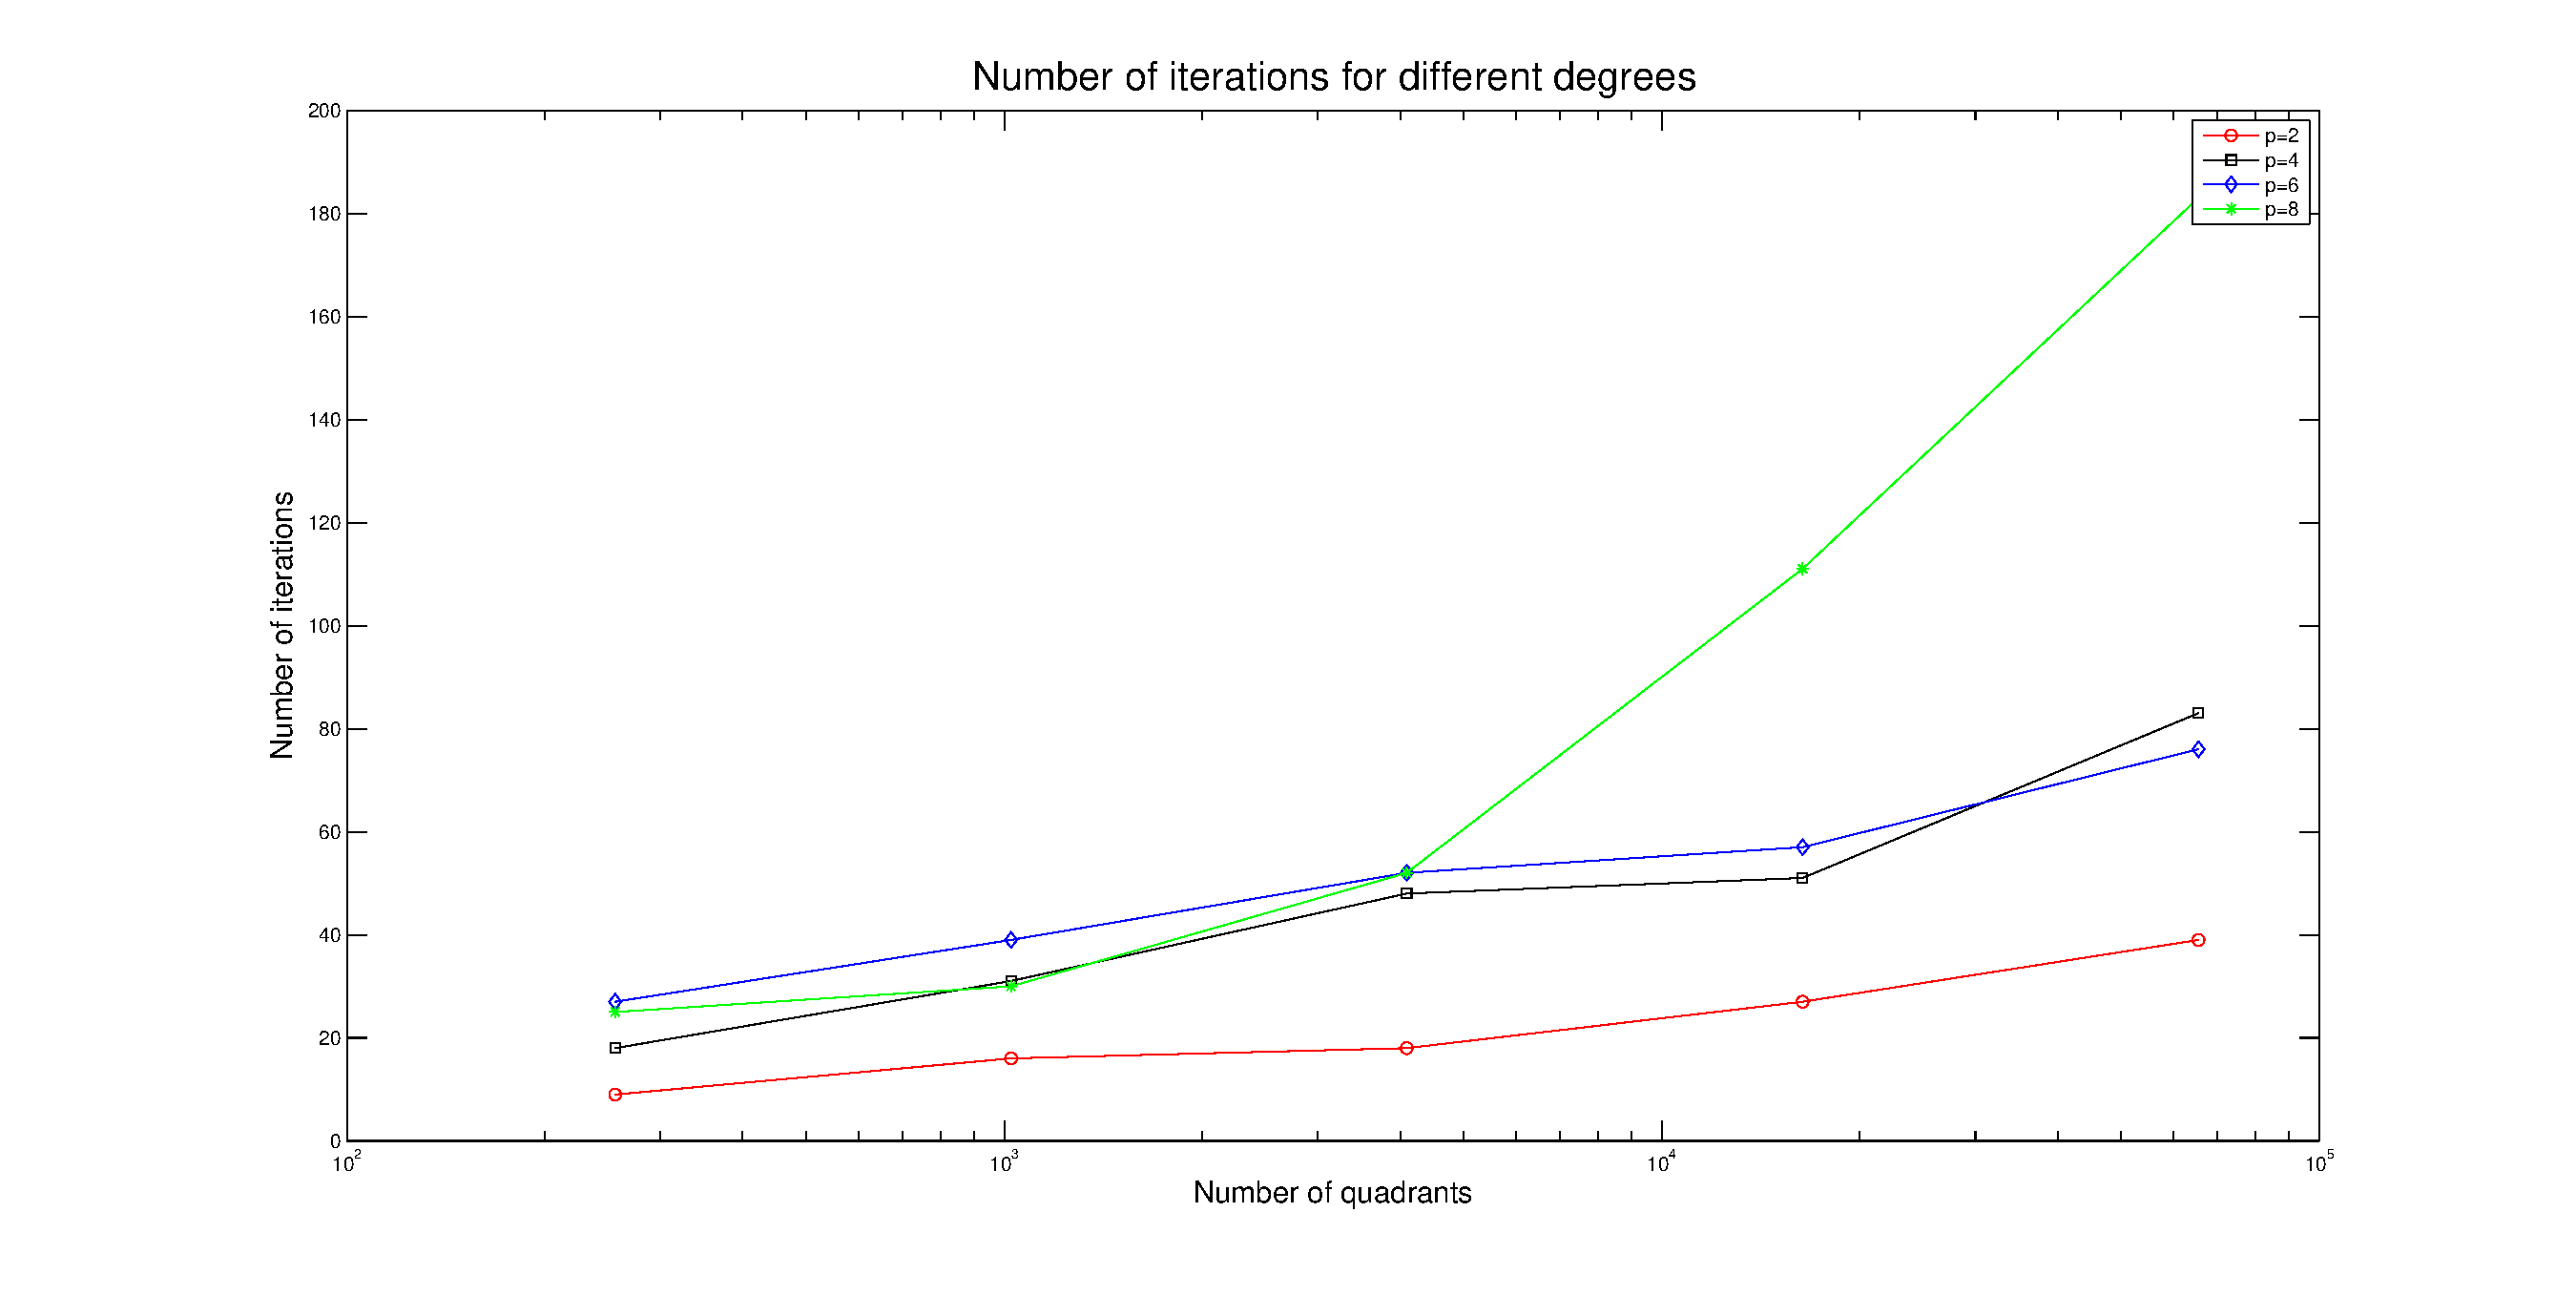
\includegraphics[scale=0.35]{Results/fine_reg_iter.eps}
\caption{Number of iterations of PCG with only the fine preconditioner for different degrees $p$ of interpolation as a function of the number of quadrants in a regular mesh.}
\label{fine_reg_iter} 
\end{figure}

We can see that, even without the coarse preconditioner, we are solving the system in a small number of iterations compared to the number of degrees of freedom. For example, we only do about 80 iterations to solve the system with $2.4\: 10^{6}$ degrees of freedom and with interpolations of degree $p=6$. 

 We can also see that for every degree, the number of iterations increases when we refine the mesh. This is to be expected since the information from the boundaries has to go through more quadrant before propagate to the entire domain. Asymptotically, the number of iterations is expected to double as the number of quadrants is multiplied by four (i.e. the mesh size is divided by two). We can see that it is not yet the case here.

A last remark we can make is that the number of iterations tends to increase when the degree of the interpolation increases. This is especially true for the finest mesh where we need 183 iterations for $p=8$ where we only need 39 iterations for $p=2$. This can be explained by the fact that the size of the overlap decreases when $p$ grows. As mentioned in \cite{overlap_constant}, this issue would be fixed if we imposed a constant overlap.

\subsubsection{Meshes with distorted elements}
Let us now move on to meshes that are not regular anymore. Let us remember that when we developed the fine preconditioner, we assumed that the elements were rectangular which allowed us to compute the analytic solution to the problem. This part explores the influence of having distorted elements on the number of iterations needed to obtain a given accuracy. 

\begin{figure}
\centering
\begin{subfigure}{.5\textwidth}
  \centering
  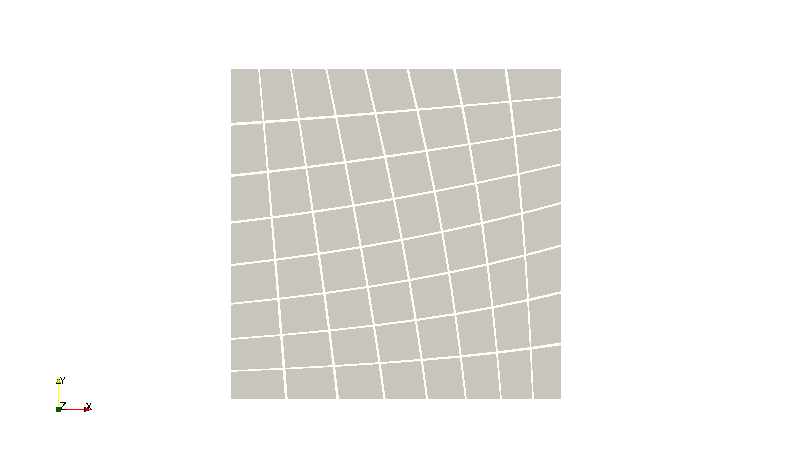
\includegraphics[width=1.2\linewidth]{Results/fine_mesh_deform_1.png}
  \caption{Mesh with $a=1.1$}
  \label{fine_mesh_deform_1}
\end{subfigure}%
\begin{subfigure}{.5\textwidth}
  \centering
  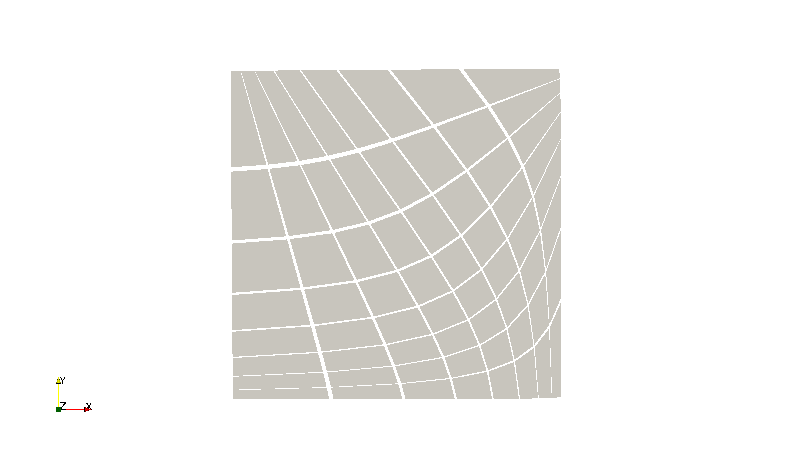
\includegraphics[width=1.2\linewidth]{Results/fine_mesh_deform_2.png}
  \caption{Mesh with $a=1.4$}
  \label{fine_mesh_deform_2}
\end{subfigure}
\caption{Examples of the meshes used for the tests of the fine preconditioner with distorted elements. The meshes are created using GMSH with its progression tool. The key parameter is the common ratio $a$ that we will be increasing progressively.}
\label{fine_mesh_deform}
\end{figure}

To control the deformation, we will continually deform the regular mesh using the progression tool of GMSH (information about GMSH can be found in \cite{gmsh}, or in \cite{gmshPaper}). The deformation is performed using a geometric progression, with the common ratio $a$ as the parameter. Obviously, the higher the parameter $a$, the more distorted the mesh is. It is clear that for $a=1$, we have a regular mesh. Figure \ref{fine_mesh_deform} presents two meshes of obtained with the progression with GMSH. On the left we used $a = 1.1$ and on the right we used $a=1.4$. 

Using the same tolerance as in the previous part, we ran the preconditioned conjugate gradients with the fine preconditioner for those new meshes. The order of the interpolation used is $p=2$. The results are given in figure \ref{fine_dist_iter}.

We can see, as it was expected, that the more we deform the mesh, the more iterations we need to do in order to obtain the wanted accuracy. The fact that, for distorted elements, we do not invert exactly the system but use an approximation allows us to compute the fine preconditioner efficiently even when we have a lot of elements but we can see here that it also costs more iterations of the preconditioned conjugate gradients. However, the gain is still huge. Indeed, for a degree of interpolation $p$, we have $(p+3)^2$ nodes per overlapping subdomain. This means a complexity of $\mathcal{O}((p+3)^6)$ to solve the system exactly. Instead, with the method we use, we only need to do a few matrix multiplications where the matrices have $(p+3)$ rows and columns. This means a complexity of $\mathcal{O}((p+3)^3)$. Even with $p=2$, the results show that it is much faster to not take geometric factors into account. 

We can also note that the effect of increasing the number of elements (i.e. reducing the mesh size) on the number of iterations is clearer here. For example, for the mesh with $a = 1.15$, we need 10 iterations for $8^2$ elements, 18 iterations for $16^2$ elements and 39 iterations for $32^2$ elements. The same explanation applies here : when we multiply the number of elements by four, we roughly multiply the number of quadrants in each direction by two and therefore the information needs twice as many iterations to propagate to the domain. 

\begin{figure}
\centering
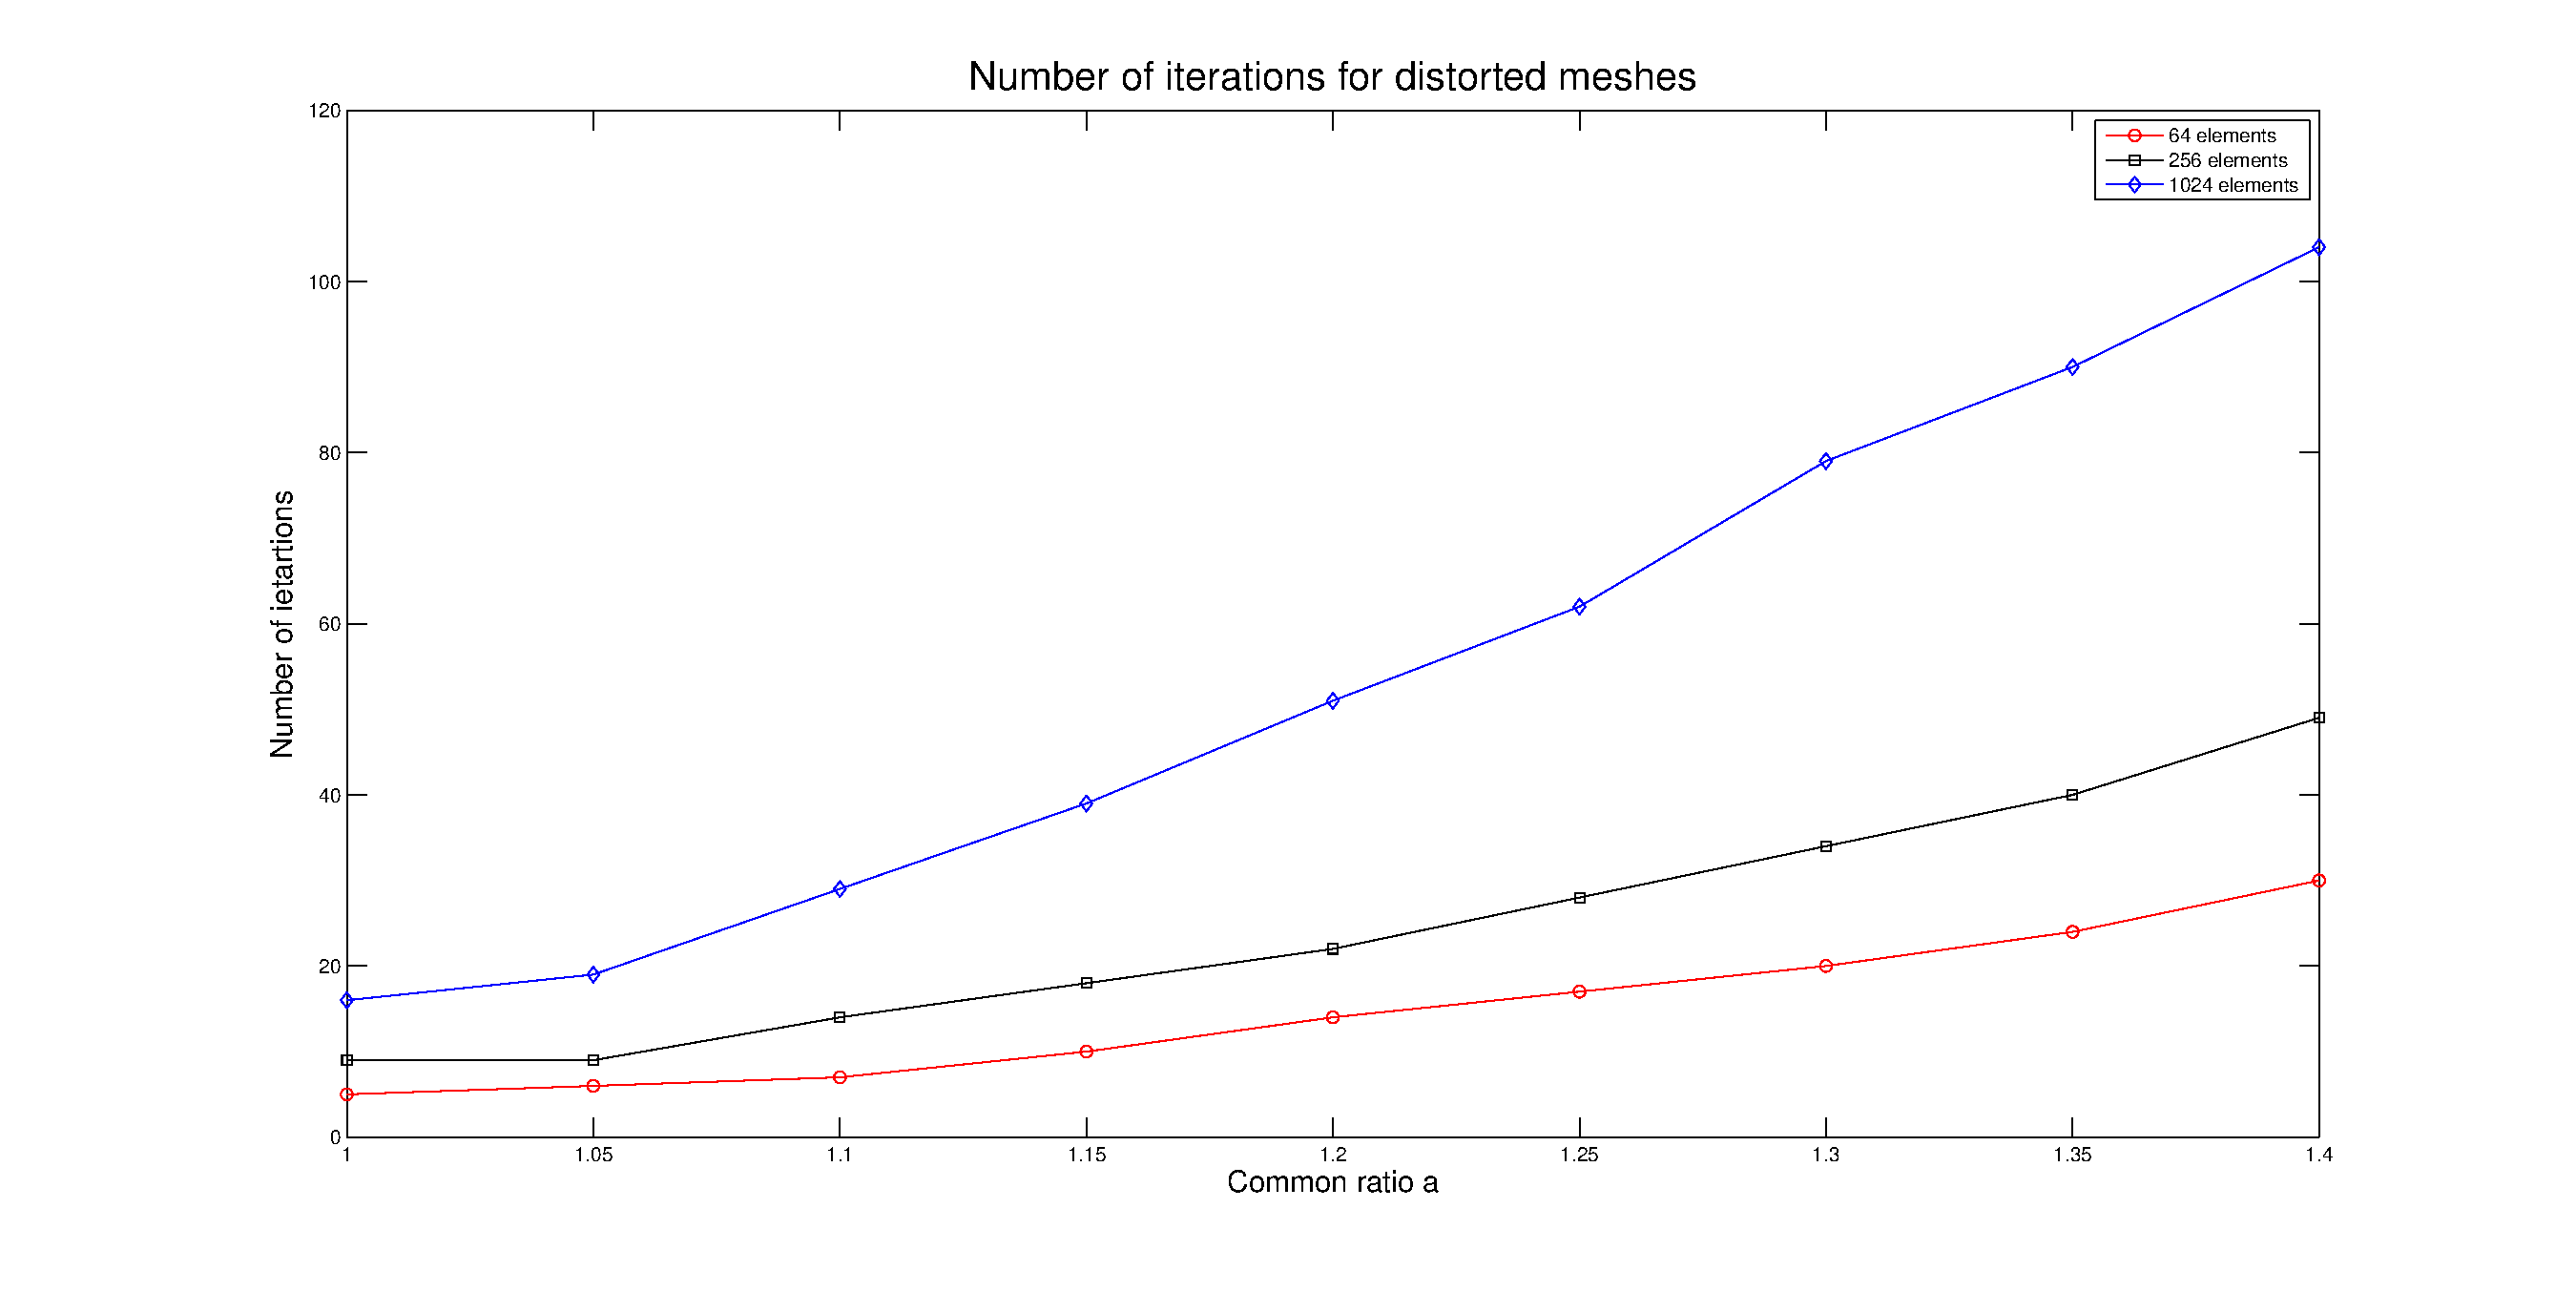
\includegraphics[scale=0.35]{Results/fine_dist_iter.eps}
\caption{bla}
\label{fine_dist_iter}
\end{figure}



\subsection{Influence of hanging nodes}
 In this part, we will explore the influence of hanging nodes on the number of iterations needed by the preconditioned conjugate gradients with the fine preconditioner to converge. Because we want meshes that are not artificial and come from real AMR applications, we will change the forcing term in this part and we will also use a recursive refine function when we build the mesh with p4est. 
 
 Let us first define the problem and the forcing term. As before, the domain is : $\Omega = [-1;1]^2$ and $\Gamma$ is the boundary. We will solve : 
 
 \begin{align}
 \nabla^2 u &= -2\tanh(nx)\tanh(my)\left[ n^2(1-\tanh(nx)^2) + m^2(1-\tanh(my)^2)\right] &\text{on $\Omega$} \label{eq:prob3}\\
u &= \tanh(nx)\tanh(my)  &\text{on $\Gamma$}
 \end{align}
 
 We can see that problem \ref{eq:prob3} has an analytic solution that is given by :
 
 $$u(x,y) = \tanh(nx)\tanh(my)$$
 
 The parameters $n$ and $m$ can be adjusted to make the jump in the hyperbolic tangent steeper. An example of a numerical solution with $p=1$ and obtained by our multigrid solver has already been shown on figure \ref{multi_simple_sol} for $n=3$ and $m=3$. 
 
 As explained before, we will use a recursive refine function when we build the forest. Since we know the analytic solution, we can cheat a little and use it for the refinement process. We will ask that the absolute value of the difference between the value of $u$ in the center of the quadrant and the mean of the values of $u$ at the four corners of the quadrant is less than a fixed tolerance multiplied by the maximum value of the function. So, if the four corners have coordinates $(x_i , y_i)$ for $i=0,1,2,3$, and that $u_{max} = max_{x,y \in \Omega} \left| u \right|$, we impose the following rule :
 
\begin{align}  
  \left| u(\frac{1}{4}\sum_{i=0}^3 x_i , \frac{1}{4}\sum_{i=0}^3 y_i) - \frac{1}{4}\sum_{i=0}^3 u(x_i,y_i)\right| < u_{max} tol
  \label{hang_rel}
\end{align}
  
Where $tol$ is a fixed tolerance. Intuitively, the tighter the tolerance, the more refined the grid needs to be and the more hanging nodes we will have thanks to the jump in the hyperbolic tangent function. 

\subsubsection{Increasing the relative number of hanging nodes}

To have a rather steep jump, we chose $n=m=12$ for the different tests that follow. We varied the tolerance to have more or less hanging nodes. We also needed a way to quantify the presence of hanging nodes. Let us define $hang$, the ratio of the number of hanging nodes over the number of global nodes. 

\begin{align}
 hang = \frac{\#\text{hanging nodes}}{\#\text{global nodes}}
 \label{hang_frac}
 \end{align}

\begin{table}
\centering
\begin{tabular}{c|ccc}
\hline
Tol & 0.020 & 0.015 & 0.010\\
\hline
Number of quadrants &1276 & 1384 & 3064 \\
\hline
hang & 14.05\% & 16.61\% & 22.13\%\\
\hline
\end{tabular}
\caption{Number of quadrants obtained using the recursive refine function on the problem \ref{eq:prob3} for different tolerances as well as the ratio $hang$ for each mesh with an interpolation of degree $p=2$.}
\label{fine_hanging_ratio}
\end{table}

Table \ref{fine_hanging_ratio} shows this number for different values of the tolerance and for $p=2$. We can see, as expected, that the ratio $hang$ increases while we make the tolerance tighter. Of course, the exact value of $hang$ does not matter since even for a given mesh, it will change with the degree of the interpolation so it is rather how it evolves that interests us. 

\begin{figure}
\centering
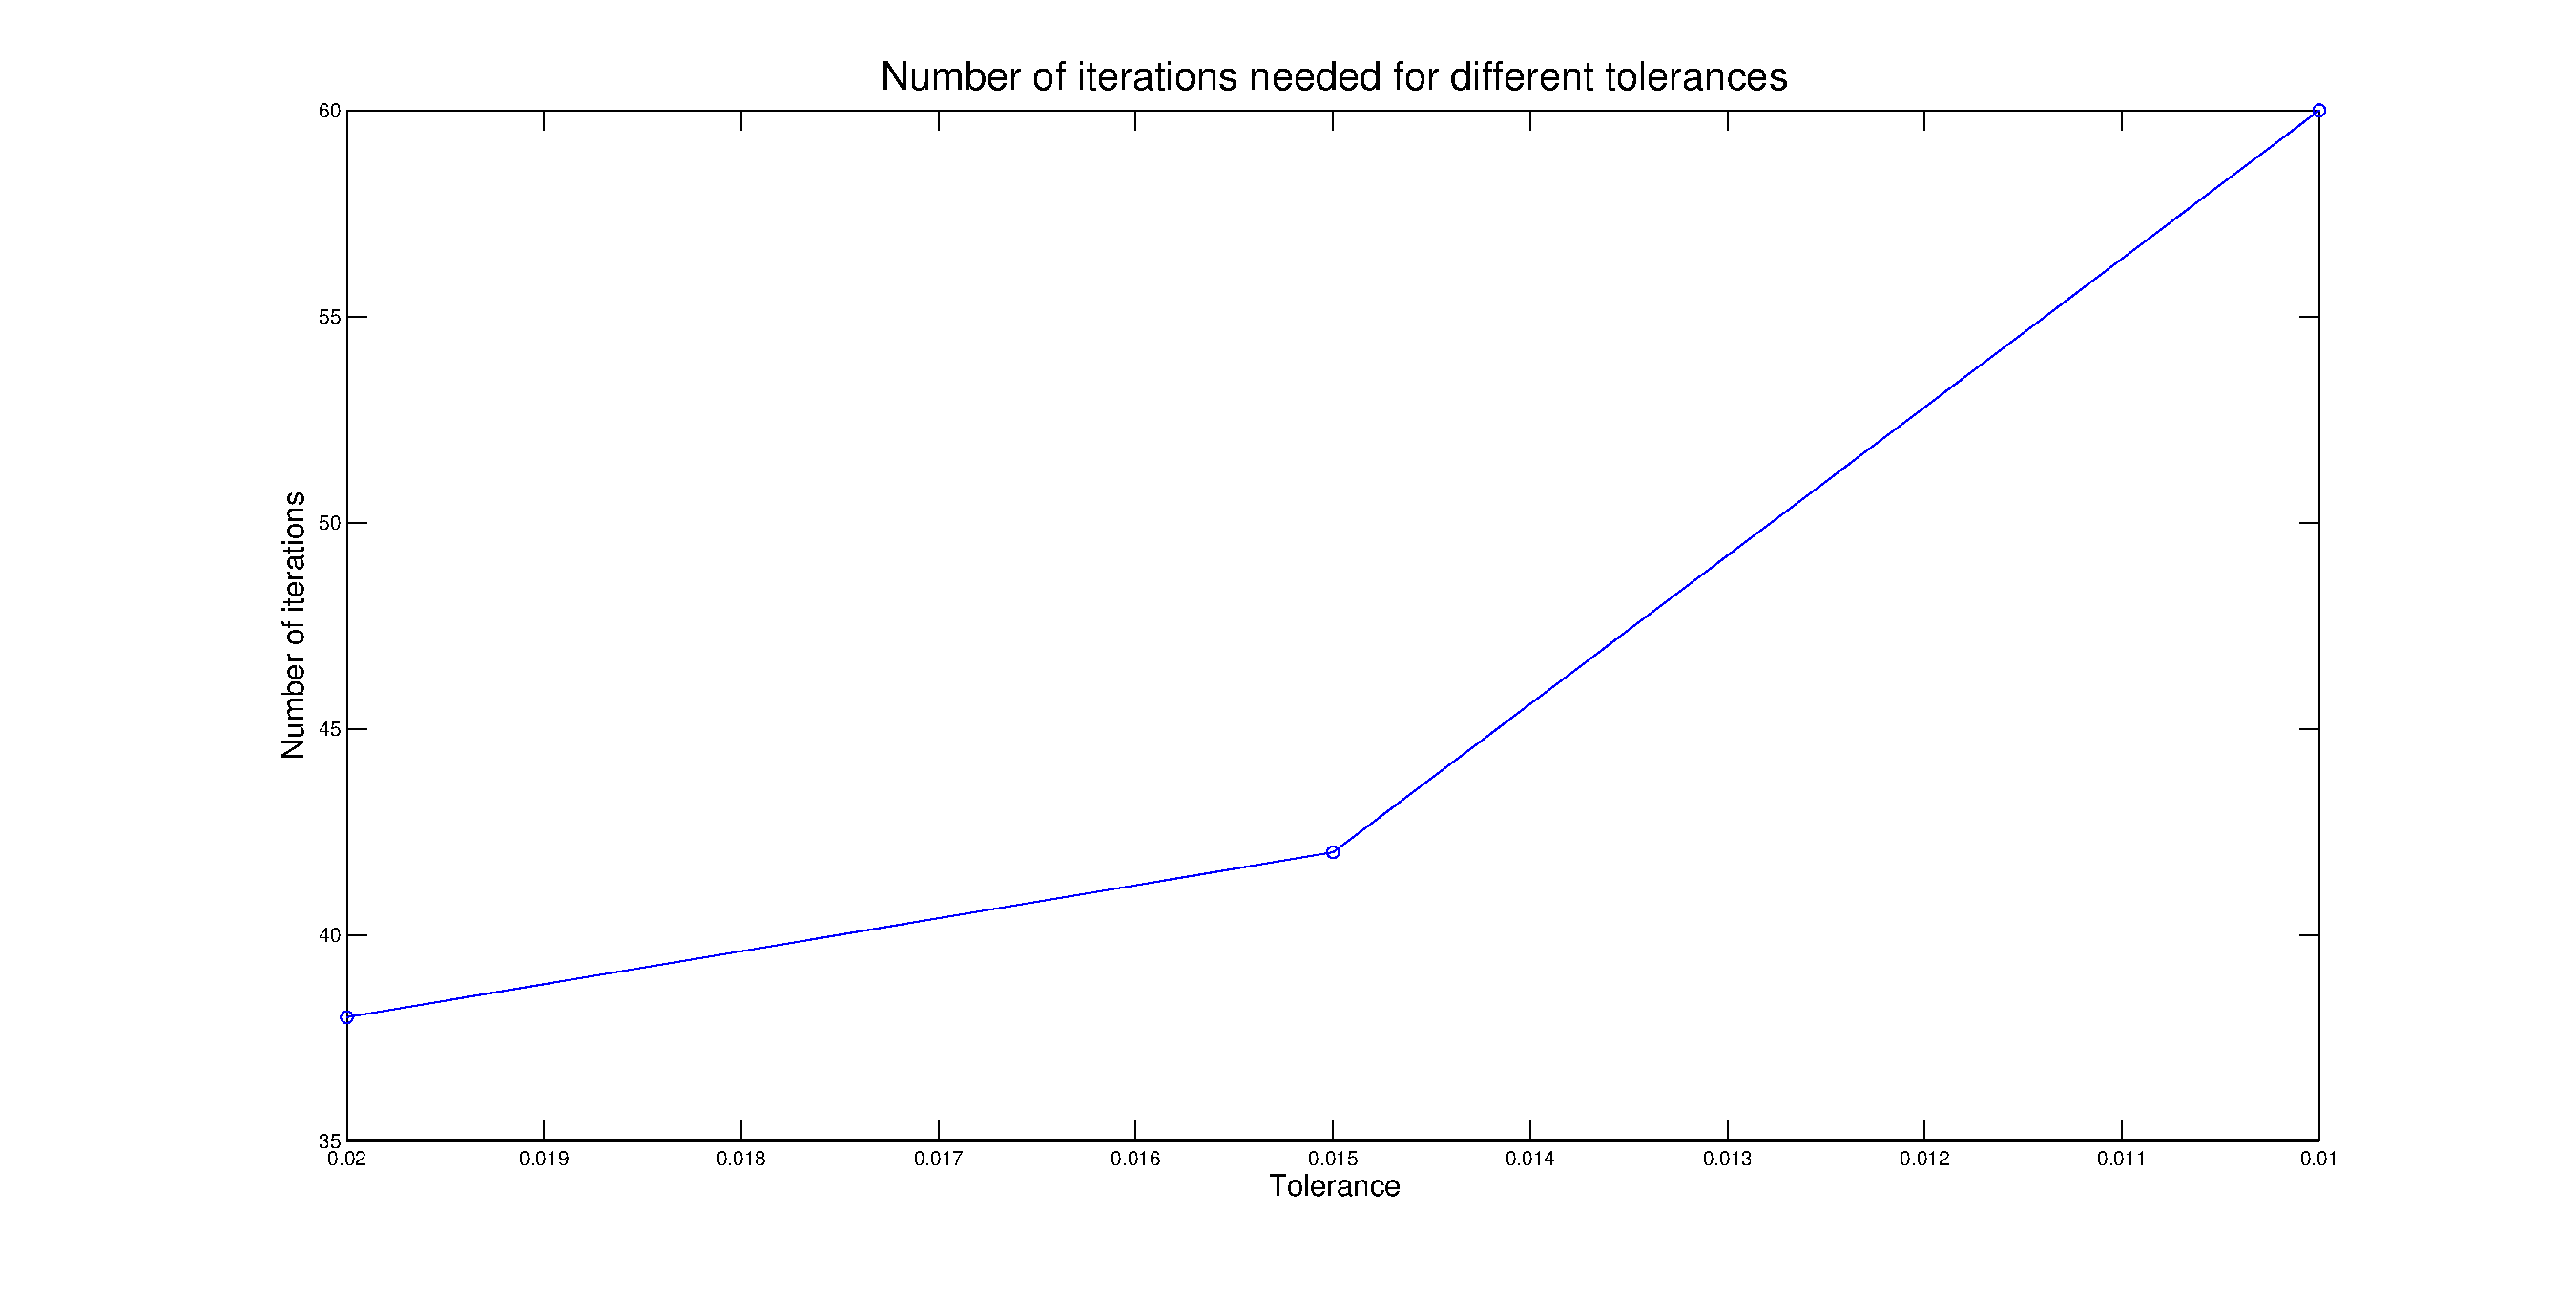
\includegraphics[scale=0.35]{Results/fine_hang_plot.eps}
\caption{Number of iterations needed to reach a given norm on the residual for a degree of interpolation $p=2$ and for meshes obtained with different tolerances.}
\label{fine_hang_plot}
\end{figure}


Let us now see how the number of iterations varies for the different meshes. Figure \ref{fine_hang_plot} shows the number of iterations needed to reach the same norm on the residual as before for the three different meshes obtained with the tolerances presented in table \ref{fine_hanging_ratio}. We can see on the graph that the number of iterations increases when we have relatively more hanging nodes. We have to be careful since this phenomenon can also be explained by the fact that we have more quadrants when the tolerance gets tighter and that also causes an increase in the number of iterations as showed earlier in this section. However, it is observed that we need less iterations when we do not have hanging nodes and for a similar number of quadrants (for example, for 1024 quadrants without hanging nodes, we need 18 iterations whereas we need 38 for 1276 quadrants). 


As explained in the implementation chapter, when we have hanging nodes, we do not treat all hanging possibilities and therefore we have an error when we compute the local residual. This explains why we need more iterations in presence of hanging nodes and the fact that we converge less quickly the more hanging nodes we have in the mesh. However, the number of iterations is still acceptable.

\subsubsection{Increasing the degree of the interpolation} 

\begin{figure}
\centering
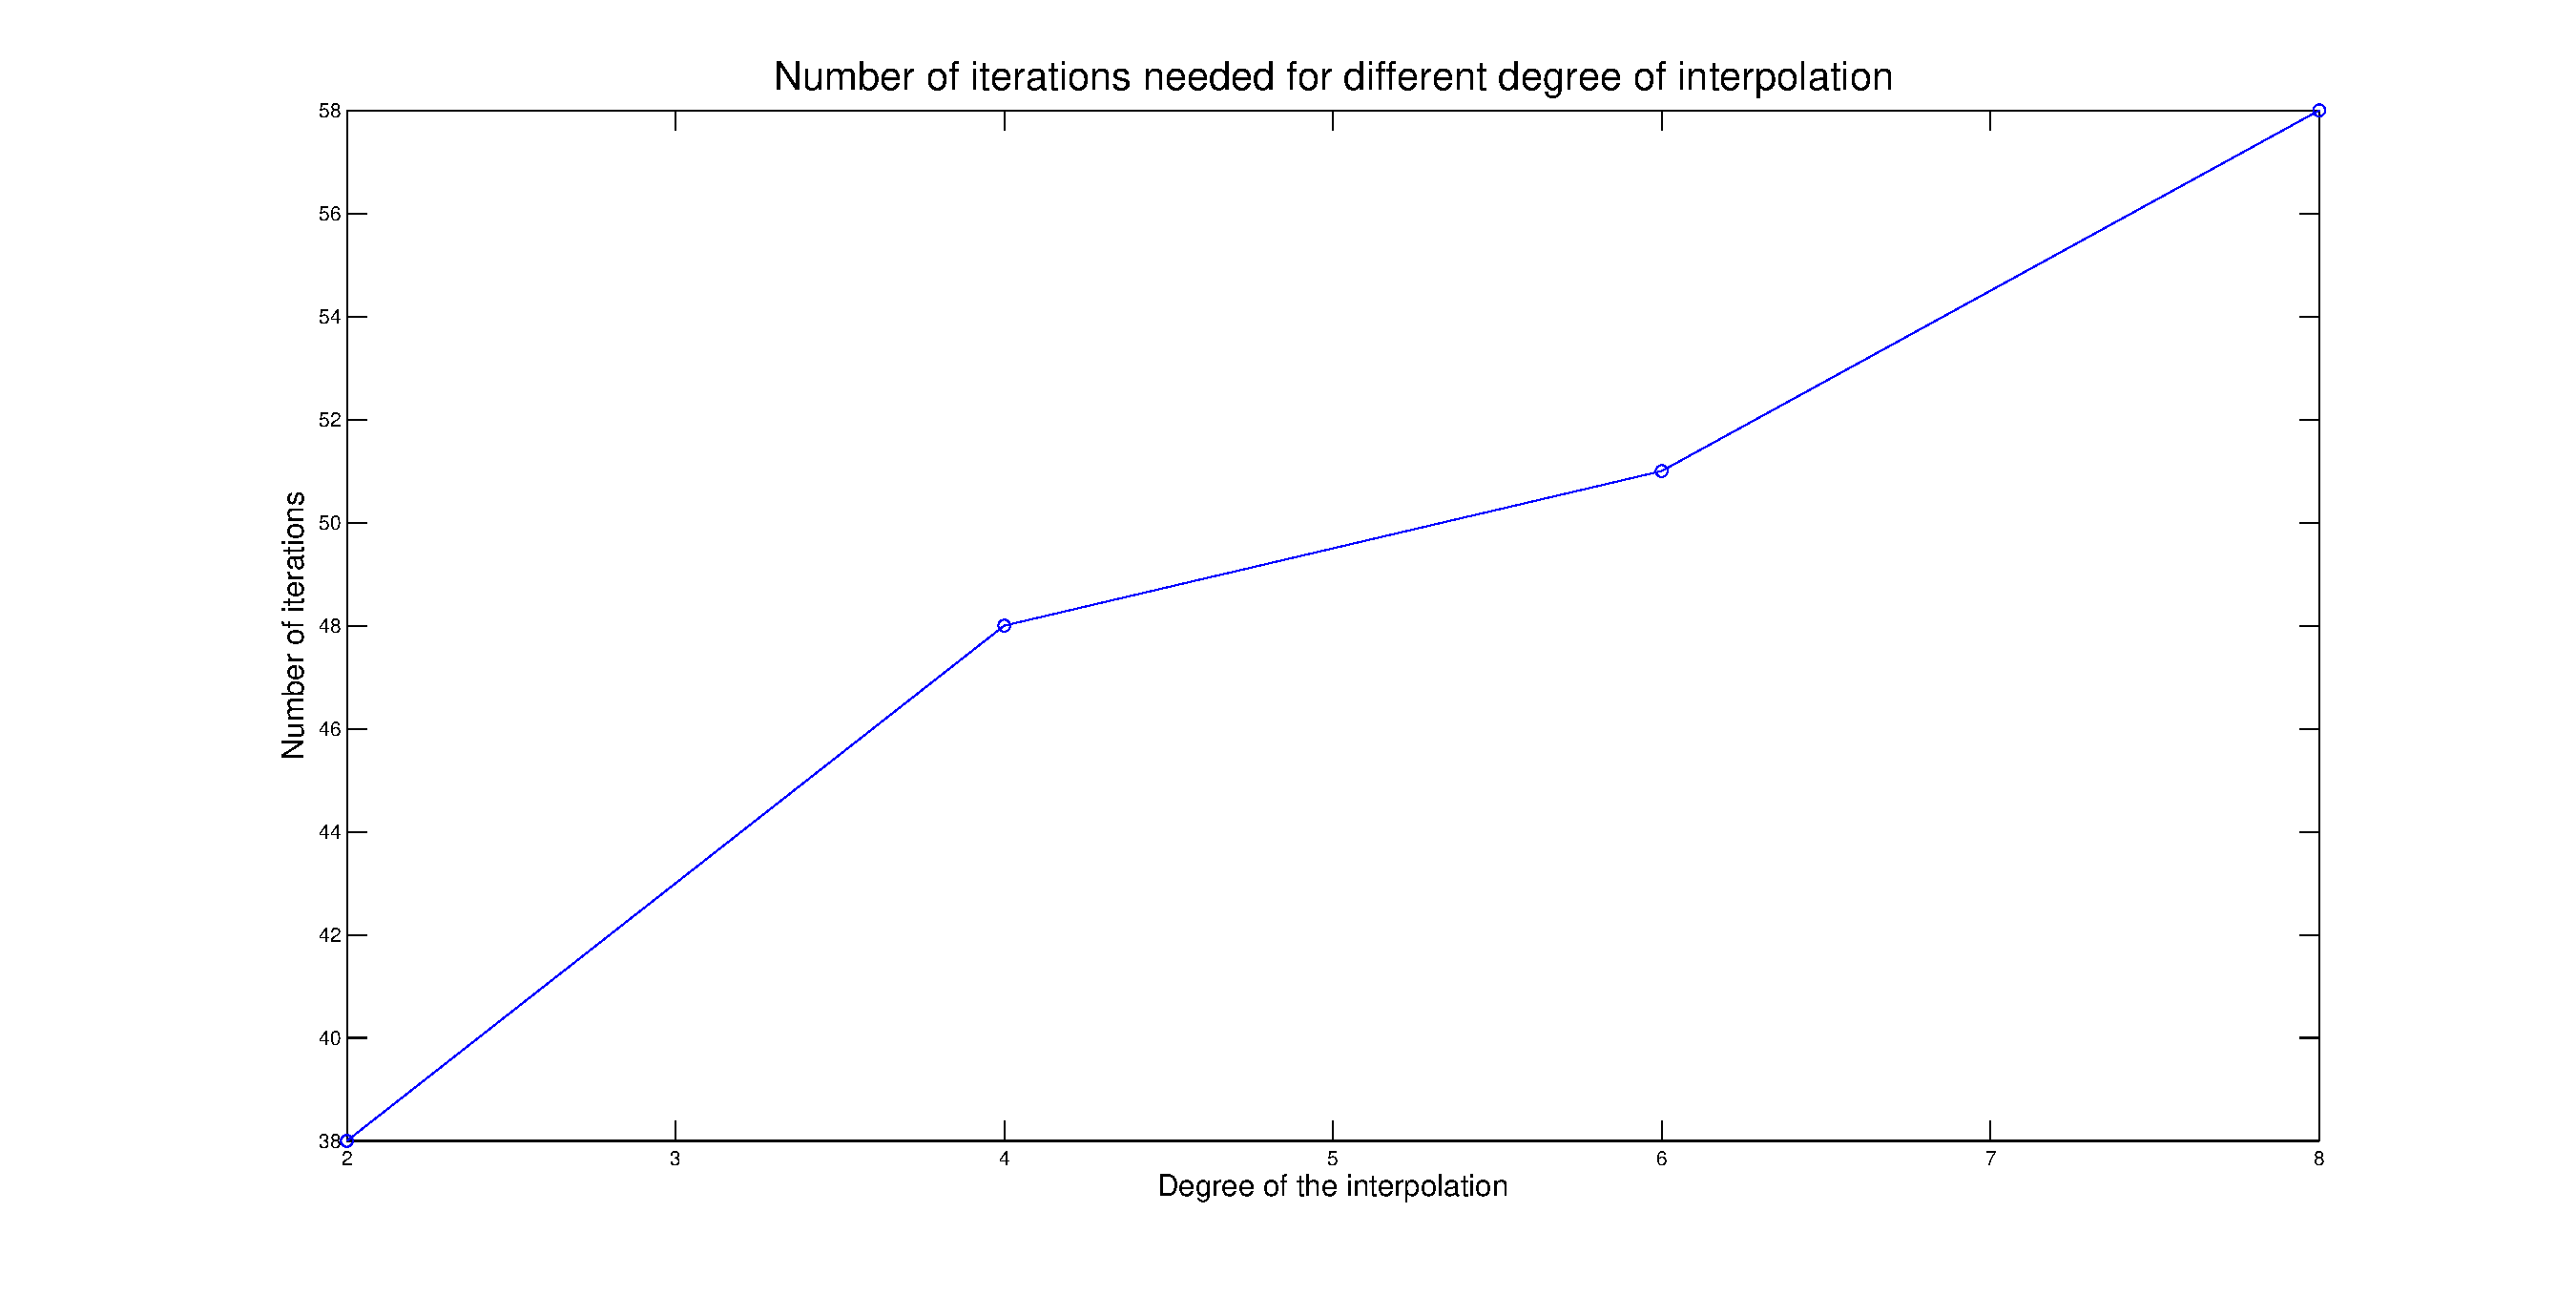
\includegraphics[scale=0.35]{Results/fine_hang_deg.eps}
\caption{Number of iterations needed to reach the tolerance of the norm of the residual as a function of the degree of the interpolation used for a mesh obtained using $tol=0.02$ in the recursive refine function.}
\label{fine_hang_deg}
\end{figure}

Let us finally look at what happens when we increase the degree of the interpolation. We tried different degrees of interpolation ($p=2,4,6,8$) and looked at the number of iterations needed to obtain the numerical solution. Figure \ref{fine_hang_deg} shows the results.  

We can see that the number of iterations increases with the degree. We need 38 iterations for $p=2$ but 58 for $p=8$. As already explained in the case with no hanging nodes, this is in part due to the fact that when we increase the degree of the interpolation, the size of the overlap decreases and therefore we need more iterations.

We can also mention the fact that since we do not treat all hanging possibilities when we compute the local residual at the overlaps, increasing the degree (and therefore the number of nodes in the overlaps) might have a effect on the number of iterations.

All the tests presented here were on meshes where the elements were not distorted and where we expect the fine preconditioner to behave optimally but the same tests have been performed with distorted quadrants and we observe the same qualitative results. 


 



 
